\subchapter{Preparing hardware}{Preparing a PC and a USB drive before
the workshop}.

Make sure the prerequisites are met before the workshop. Make sure you
do not follow the below instructions on the morning the workshop starts,
as these preparation steps can take up to several hours, depending
on the speed of your Internet connection.

Here is the required hardware:
\begin{itemize}
\item Microchip SAMA5D3x evaluation kit
\item 5V power adaptor for the kit
\item At least one USB-A (male) to micro-USB (male) cable. Two such
      cables if possible.
\item Recent PC with at least 2 GB of RAM, a decently fast processor
      and 20 GB of free contiguous space for installing Linux.
\item 1 USB flash drive with at least 4 GB of free space
\end{itemize}

\section{Installing Linux on the PC}

Do this before joining the workshop. This can be either done by
participants themselves on their own PCs, or on PCs supplied by the
entity which organizes the event.

For the practical labs in this workshop, we need you to install
{\bf Ubuntu Desktop 12.04}. We support both 32 and 64 bit variants,
though 64 bit will probably give you the best performance
if you have a recent CPU.

Get the Desktop edition of Ubuntu 12.04 at
\url{http://www.ubuntu.com/download/desktop}, and follow the
instructions. Note that Xubuntu and Kubuntu variants are fine too.

The way your disk is partition will also matter in the practical labs.
What matters is that \code{/opt} is in a partition with at least 15 GB
of disk space. It's still because of the pre-compiled build environment
which must have a specific path to be useful.

The easiest way to achieve this is to have only one big root (\code{/})
partition, which would then contain \code{/opt}. If you have enough
space, you can of course have a dedicated partition for \code{/opt}.

{\bf Important notes}
\begin{itemize}
\item We do not support Linux installations in a virtual machine.
      VMs will suffer from long compile times and will complicate
      access to the real hardware.
\item Using Ubuntu in live mode (from with installing it) will not work
      either.  Memory may get scarse, compile time will be much longer because
      of the slow disk, and exporting the root filesystem through NFS
      won't work.
\end{itemize}

At the end of installation, we recommend to install the latest updates:

\begin{verbatim}
sudo apt update
sudo apt dist-upgrade
\end{verbatim}

\section{Preparing a USB disk for the workshop}

The USB disk will be needed by workshop participants:

\begin{itemize}
\item To access files which could take a long time to download
      in the workshop venue (if it has a slow connection to the Internet
      or if there are too many people downloading the same files at
      once).
\item To get the pre-compiled build environment, saving at least
      one hour of compile time. This file is several hundreds of MB big,
      and would also take a long time to download.
\end{itemize}

Now take a USB disk with at least 4 GB of free space, and connect it
to your Ubuntu PC. You should see a window showing its contents.

We are going to reformat this disk, so that every participant
accesses his disk through the same name and path.

The first thing you need to do is find which device file is
associated to this newly inserted disk. Type the \code{dmesg} command
and look at the last lines:

\begin{verbatim}
...
[ 6103.687852]  sdb: sdb1
...
\end{verbatim}

Let's assume that this disk associated to \code{/dev/sdb}:
\begin{itemize}
\item \code{/dev/sdb} represents the whole disk
\item \code{/dev/sdb1} represents only the first partition on this disk.
      There could be more partitions.
\end{itemize}

Now, let's format this first partition for the \code{FAT32} filesystem
(make sure you replace \code{sdb1} by the right device name, otherwise
you may destroy data on other disks!):

\begin{verbatim}
sudo umount /dev/sdb1
sudo mkfs.vfat -F 32 -n BootTime /dev/sdb1
\end{verbatim}

Now, remove your USB drive and insert it again. A file explorer window
should appear:
\begin{center}
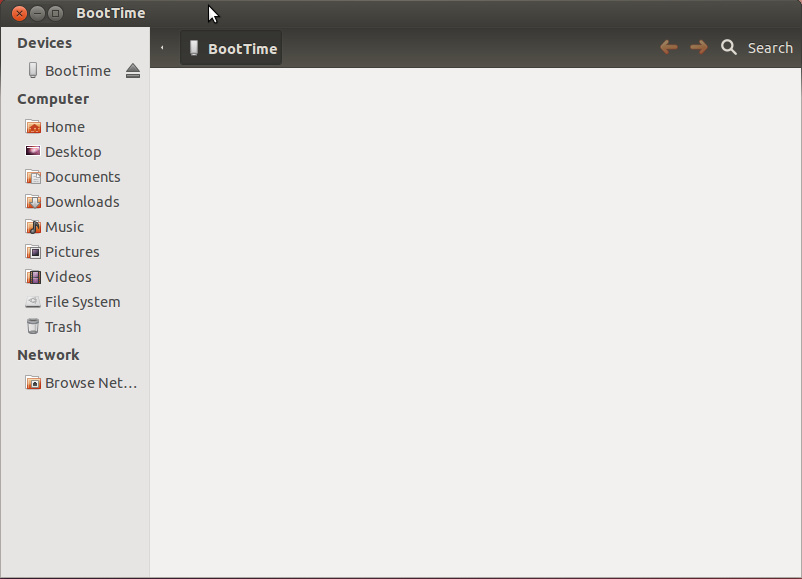
\includegraphics[width=8cm]{labs/boottime-install/usbdisk-formated.png}
\end{center}

Now let's fill this disk with data needed during the workshop:
{\small
\begin{verbatim}
cd /media/$USER/BootTime
wget -r -np -nH --cut-dirs=2 --reject "index.html*" http://bootlin.com/labs/boottime/
sudo umount /media/$USER/BootTime
\end{verbatim}
}

Depending on your Internet connection speed, downloading the files could
take up to several hours.

At the end, your USB drive contents should look like this:
\begin{center}
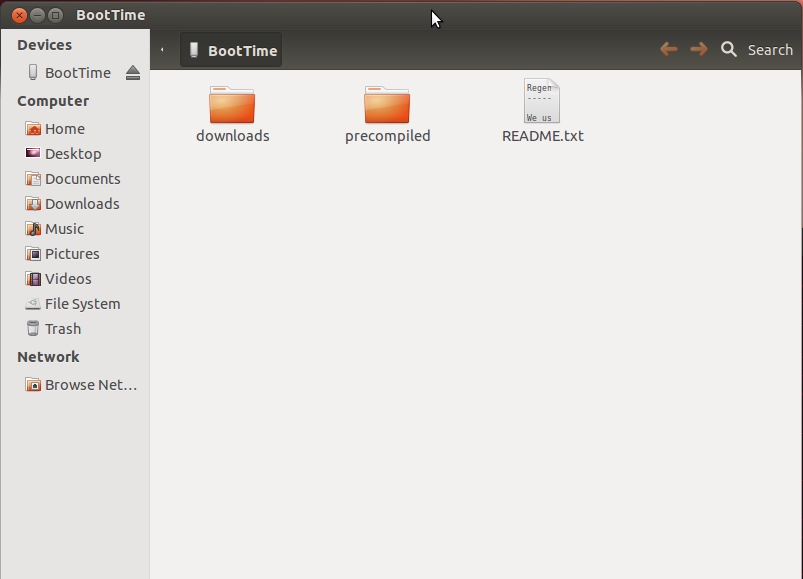
\includegraphics[width=8cm]{labs/boottime-install/usbdisk-filled.png}
\end{center}

\section{Installing the lab archive}

Please follow the below instructions carefully. If you don't use the
same directories, your pre-compiled build environment won't work and
you will waste a lot of time compiling software.

Type the below commands:
\begin{verbatim}
cd /opt
sudo chown -R $USER.$USER .
wget http://bootlin.com/doc/training/boot-time/boot-time-labs.tar.xz
sudo tar xf boot-time-labs.tar.xz
sudo chown -R $USER.$USER .
\end{verbatim}

\section{Installing software packages needed during the workshop}

This step is recommended for all workshops. It will pre-install all the
software packages needed during the workshop.

To keep our instructions as close as real life as possible, our labs
ask to install software packages exactly when they are needed. However,
if all the participants to a workshop download the same packages at the
same time, downloads are very likely to be slow.

This step can be skipped if you are just a few people doing the labs
from home or from an office with fast Internet access.

Here is the command to pre-install the software packages:

\begin{verbatim}
/opt/boot-time-labs/setup/install-packages
\end{verbatim}

\section{Ready for the workshop}

You are now ready to do the workshop!
